\documentclass{beamer}
 
\usepackage[utf8]{inputenc}
\usepackage{amsfonts, amssymb, amsmath}    
\usepackage{graphicx}
\graphicspath{ {images/} }
\usetheme{Metropolis}


\newcommand{\bX}{\mathbf{X}}
\newcommand{\bY}{\mathbf{Y}}
\newcommand{\bbeta}{\mathbf{\beta}}
 
\title[Survival of the Fittest]
{Survival of the Fittest: Variable Selection on Agricultural Data from the Gal\'apagos Islands}

\author
{Michael Bostwick}
 
\date
{April 19th, 2018}
 
 
 
\begin{document}
 
\frame{\titlepage}

\begin{frame}
\frametitle{Table of Contents}
\tableofcontents
\end{frame}
 
\section{Background}

\begin{frame}
\frametitle{Gal\'apagos Islands}
\begin{figure}
\begin{tabular}{cc}
 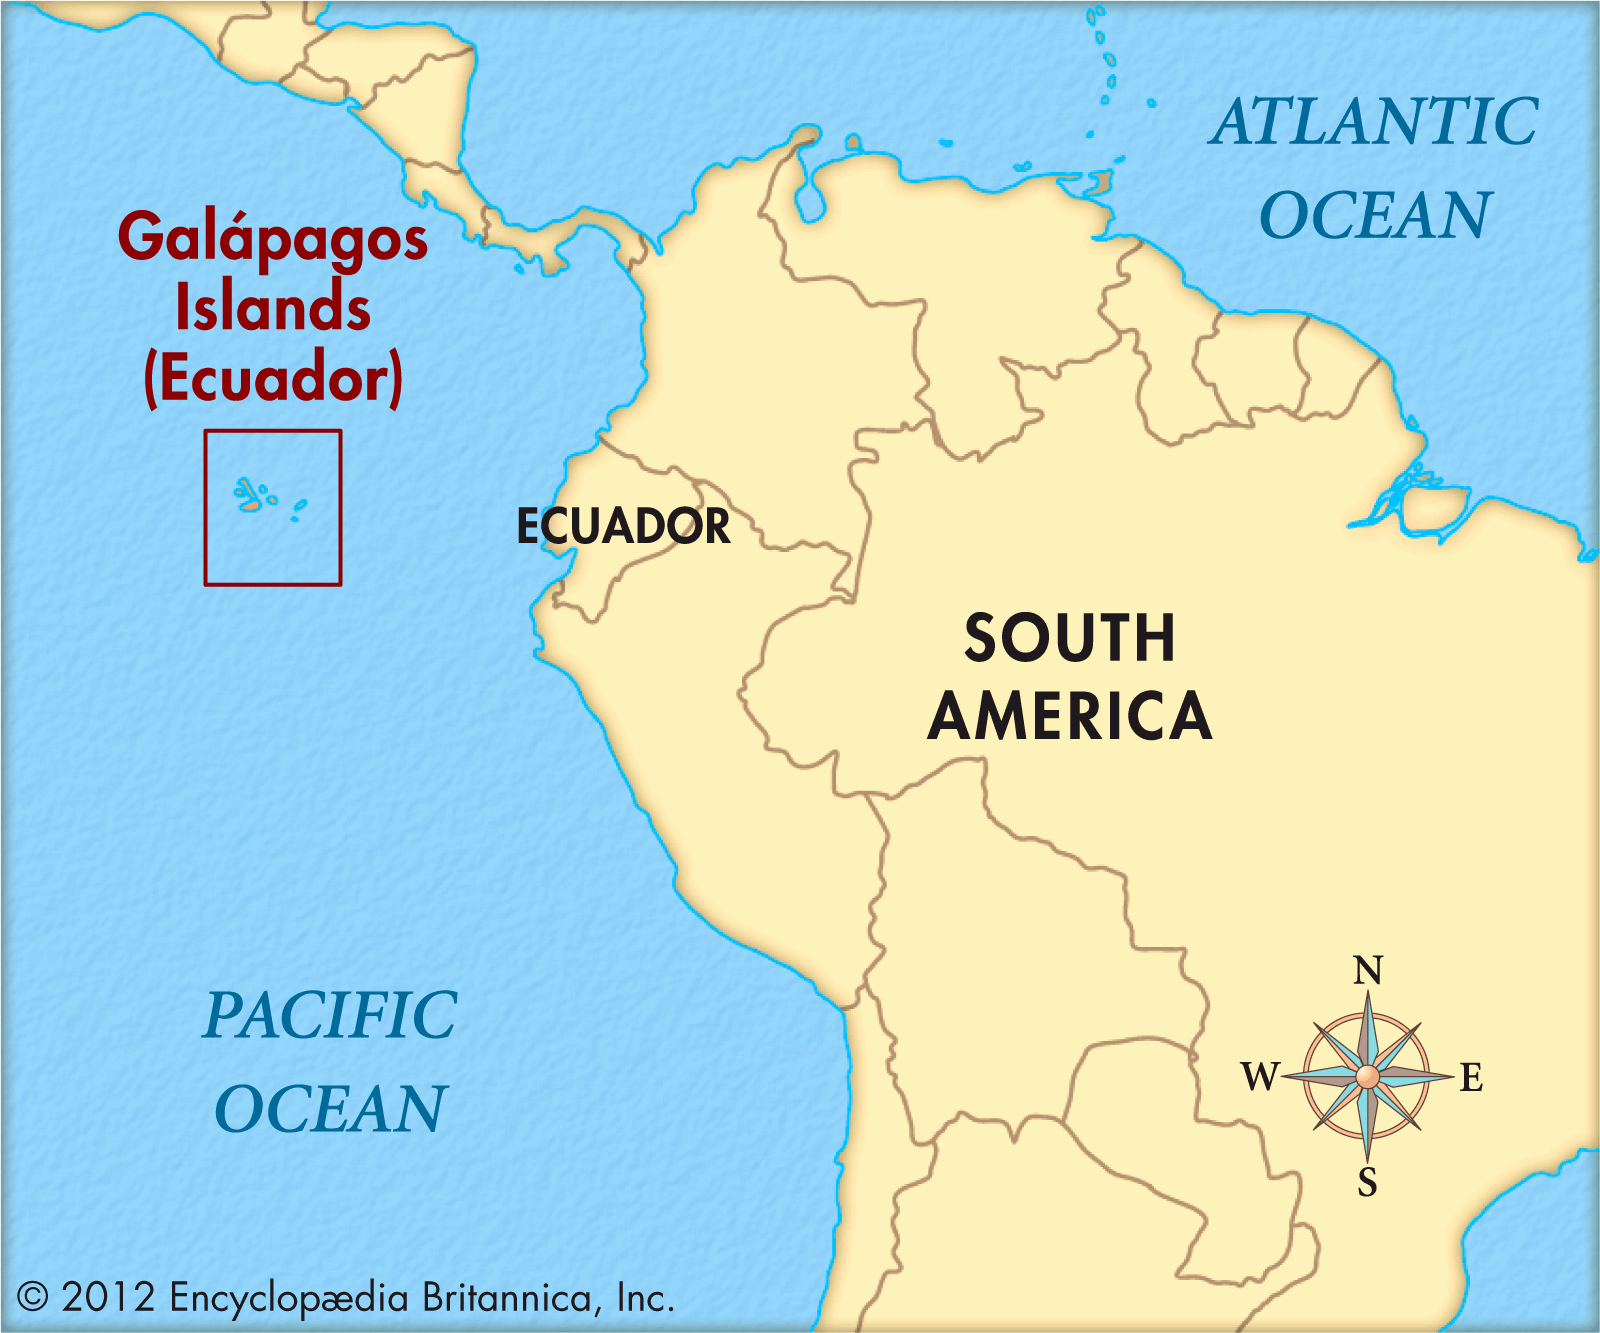
\includegraphics[scale=0.09]{galapagosmap} \footnote{https://canconf.com/map-of-south-america-including-galapagos-islands/} &   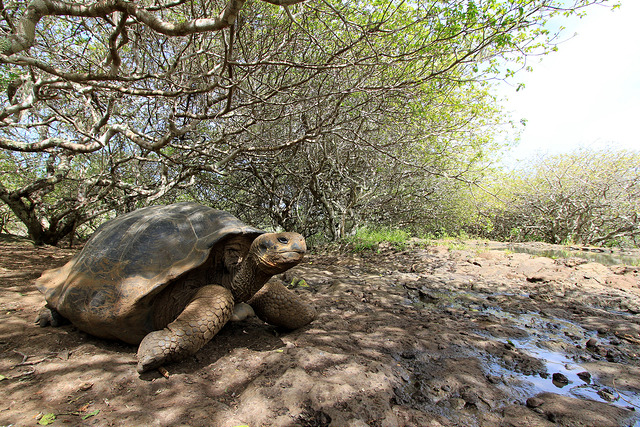
\includegraphics[scale=0.2]{turtle} \footnote{https://www.flickr.com/photos/pancholp/albums} \\
 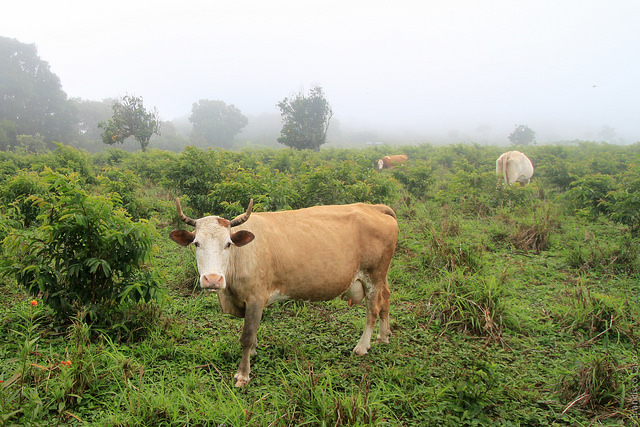
\includegraphics[scale=0.2]{cow1} &   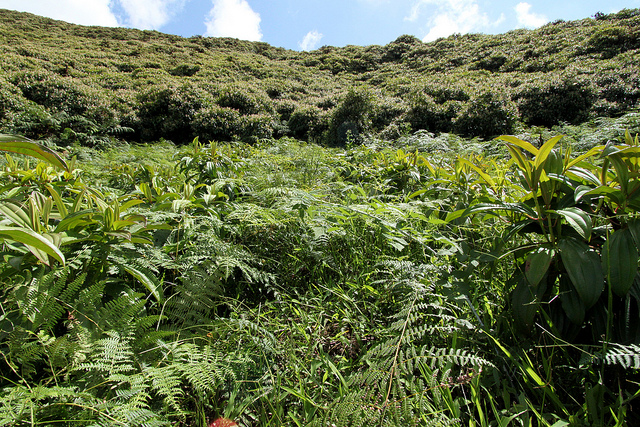
\includegraphics[scale=0.2]{invasive}
\end{tabular}
\end{figure}

\end{frame}

\begin{frame}
\frametitle{Agent-Based Simulation}
\centering
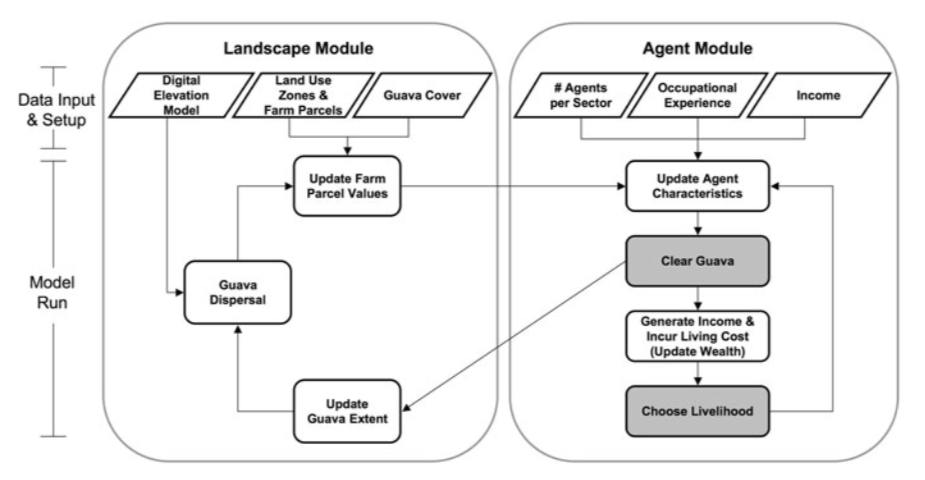
\includegraphics[scale=0.3]{abm_chart} \footnote{Miller, B. W., Breckheimer, I., McCleary, A. L., Guzm\'an-Ramirez, L., Caplow, S. C., Jones-Smith, J. C., \& Walsh, S. J. (2010). Using stylized agent-based models for population environment research: a case study from the Gal\'apagos Islands. Population and environment, 31(6), 401-426.}

\end{frame}

\begin{frame}
\frametitle{Census of Farms}
\centering

\includegraphics[scale=0.5]{survey}



\end{frame}


\section{Data}

\begin{frame}
\frametitle{Data description}
\centering
\includegraphics[scale=0.4]{755_farms}

Model 5 different response variables with 200+ possible predictors
\end{frame}

\begin{frame}
\frametitle{Data transformation}
\centering
%\[ \bY = \bX\beta + \epsilon, \epsilon \sim N(0,\sigma^2)  \]

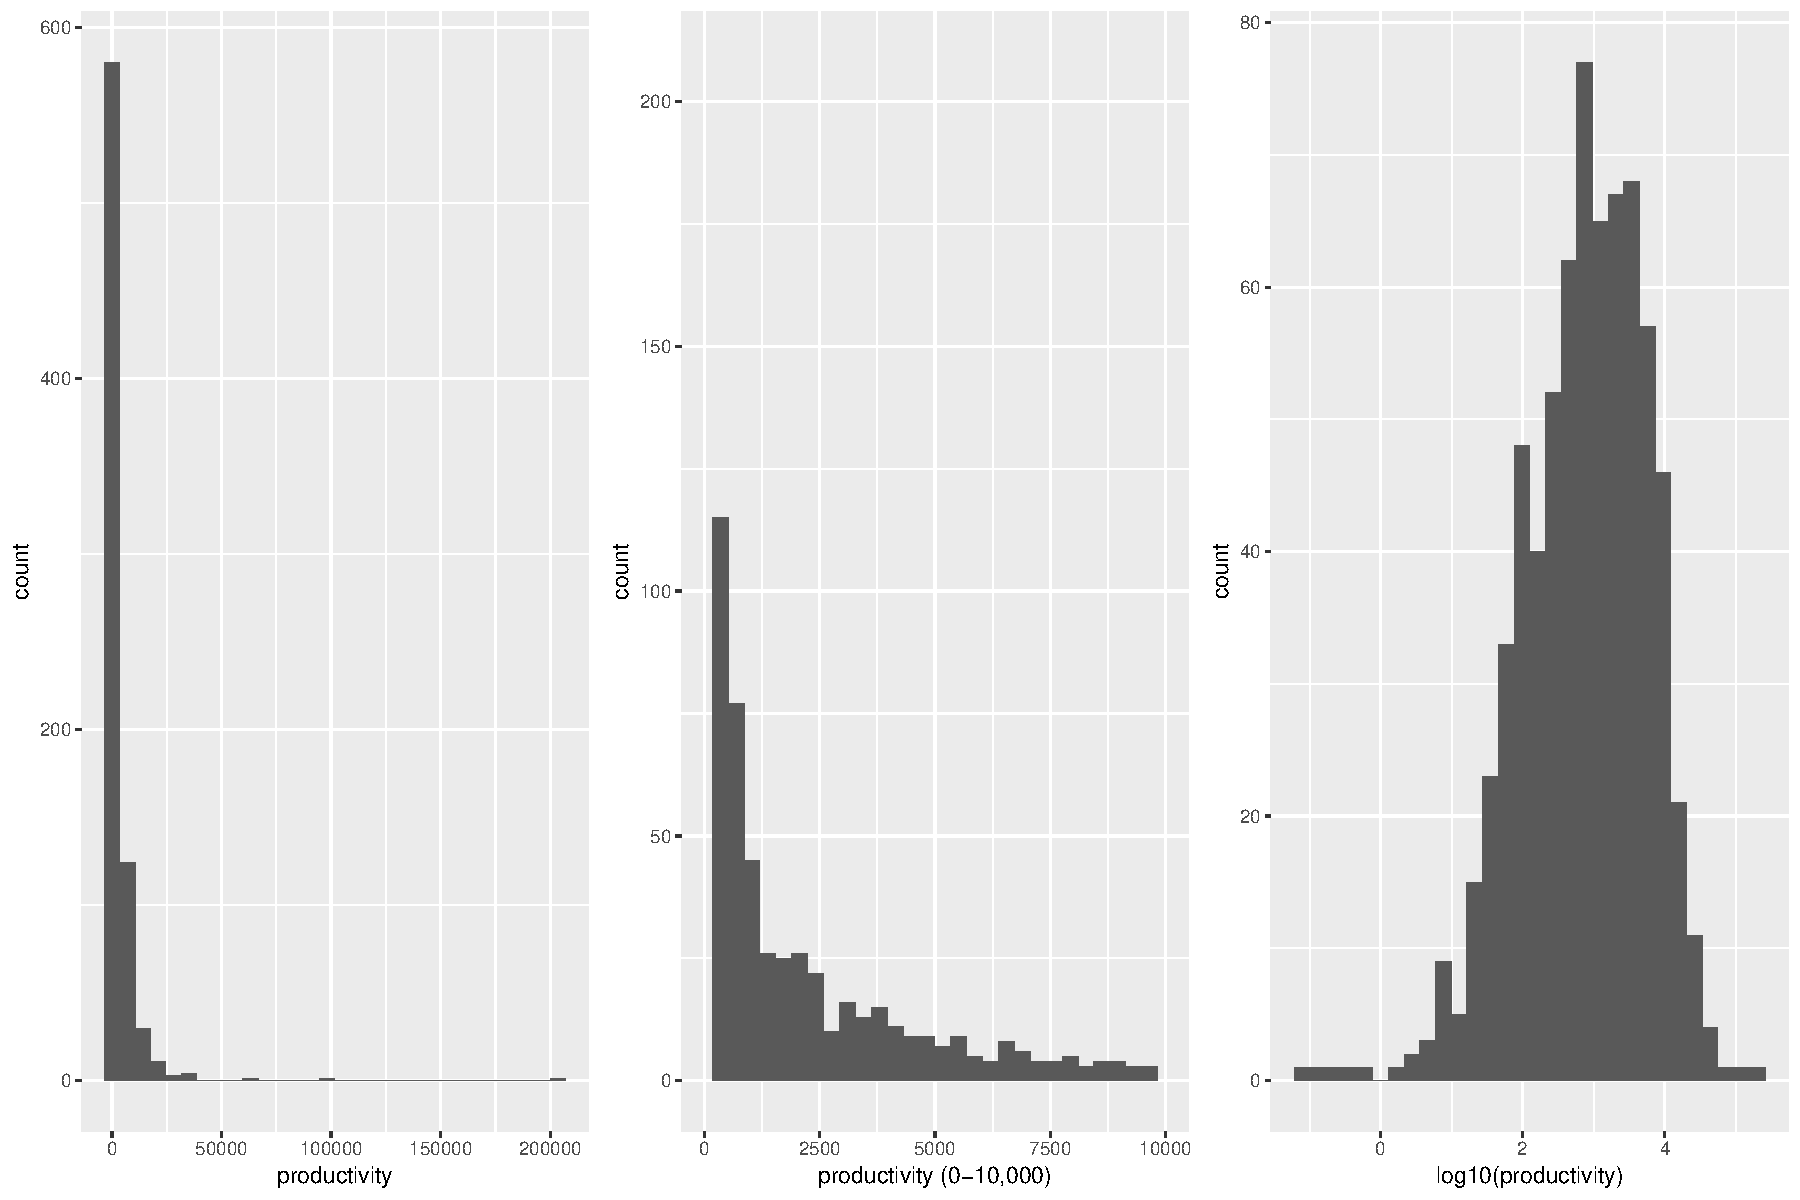
\includegraphics[scale=0.35]{production_histograms}
\end{frame}

\section{Modeling}

\begin{frame}
\frametitle{Elastic Net}

\begin{block}{Formulation}
	\[\min_{\beta}  \|\bY - \bX\beta\|_{2}^{2} + \lambda[ \underbrace{(1 - \alpha)||\beta||_2^2}_\text{Ridge} + \underbrace{\alpha||\beta||}_\text{Lasso}]\]
\end{block}

%\begin{itemize}
%	\item{Can set $\alpha$ and $\lambda$ using cross-validation}
%	\item Compromise between Ridge and Lasso can help handle correlated variables
%\end{itemize} 

\centering
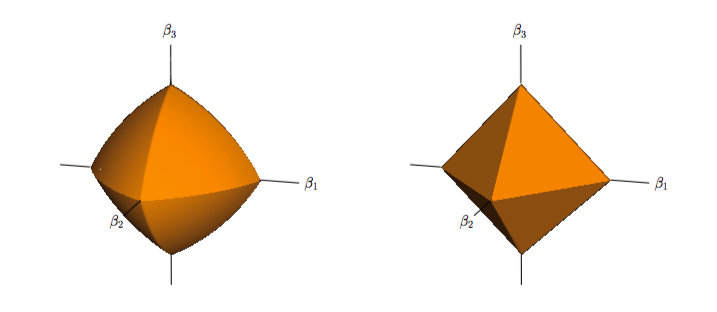
\includegraphics[width=8cm]{elastic3d} \footnote{Hastie, T., Tibshirani, R., \& Wainwright, M. (2015). Statistical learning with sparsity: the lasso and 
generalizations. CRC press.}

\end{frame}

\begin{frame}
\frametitle{Elastic Net Coefficients}
\centering

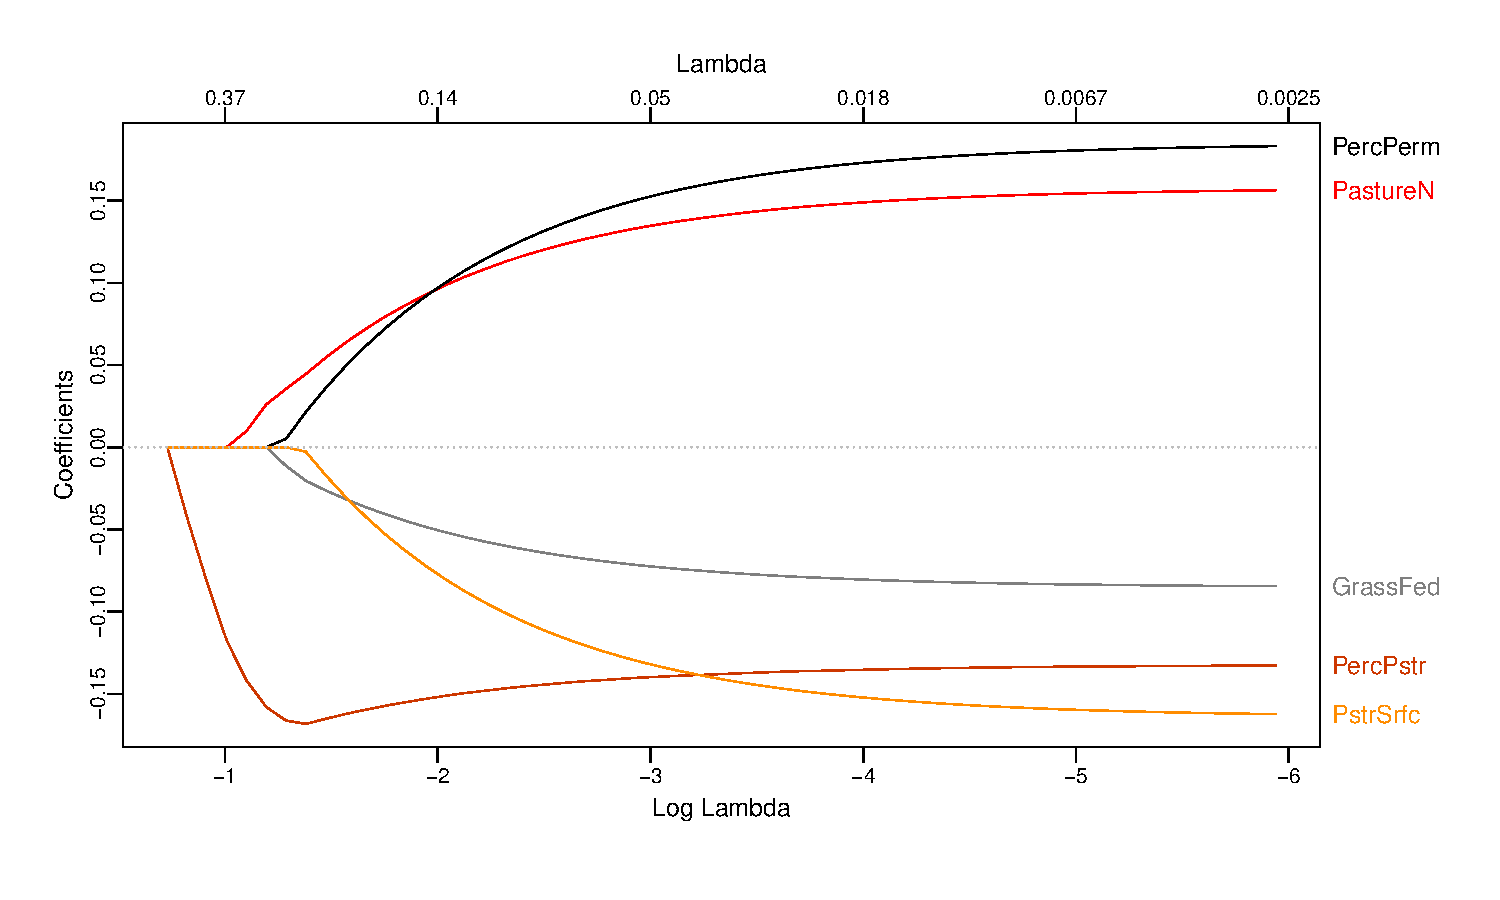
\includegraphics[scale=0.26]{elasticplot1}
Alpha = 1


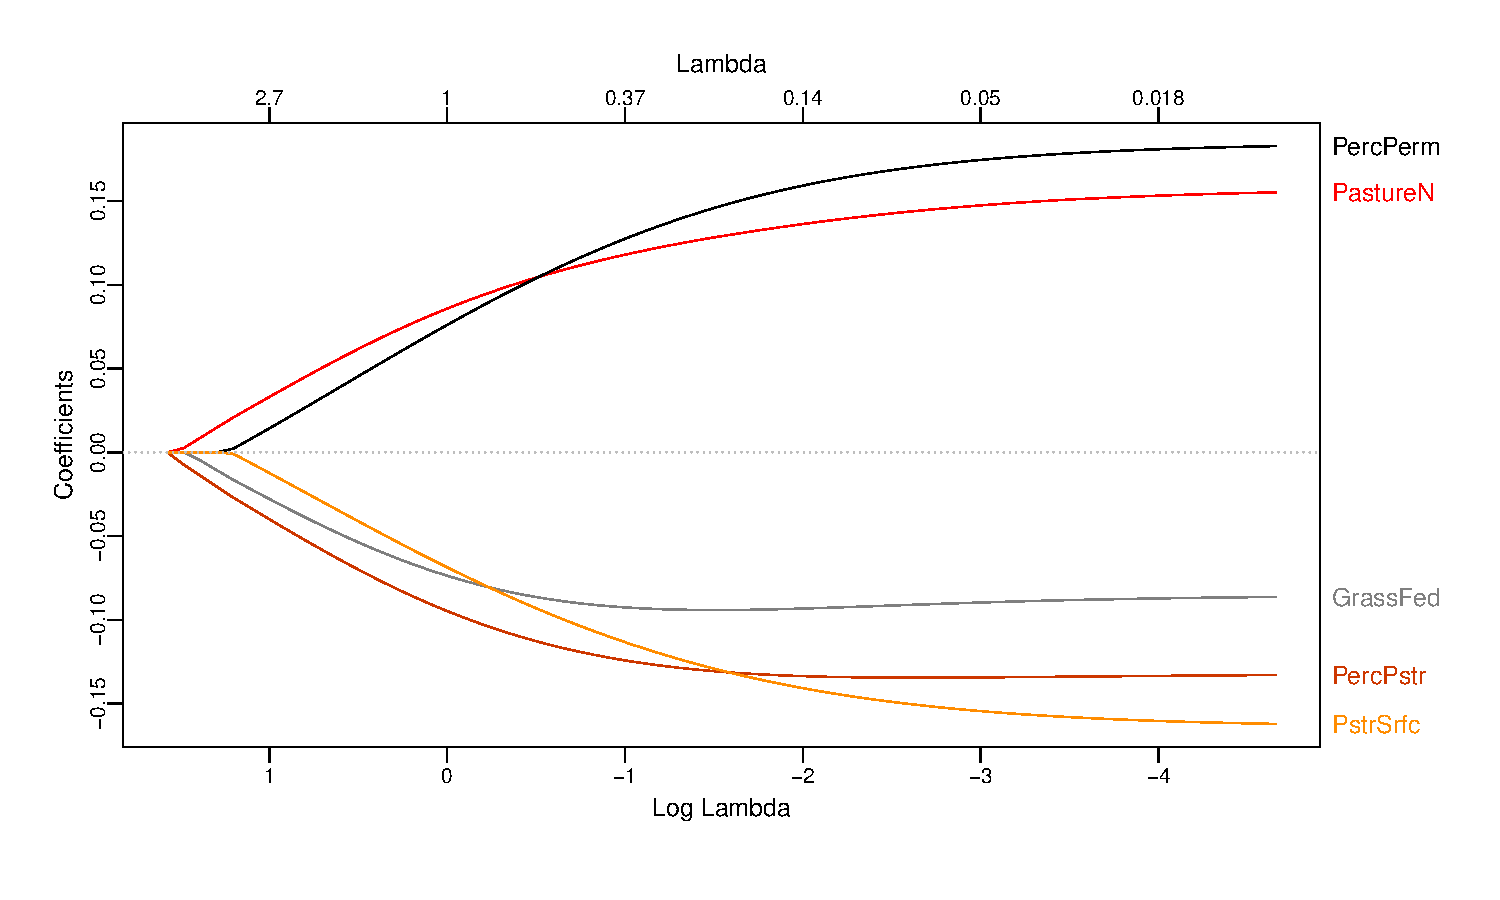
\includegraphics[scale=0.26]{elasticplot2}
Alpha = 0.1
\end{frame}


\begin{frame}
\frametitle{Forward Stepwise}

\begin{enumerate}
	\item Start with null model
	\item Fit $p$ simple linear regression models and pick one with lowest residual sum of squares (RSS)
	\item Search through remaining $p - 1$ variables and add one that best improves RSS
	\item Repeat Step 3 until all variables have been added to the model
	\item Choose optimal model using information criterion, Bayesian Information Criterion (BIC) in this case
\end{enumerate}

\[ BIC =  \frac{1}{n}(RSS + log(n)d\hat{\sigma}^2)\]

\end{frame}

\section{Results}

\begin{frame}
\frametitle{Response Variables}
\begin{itemize}
	\item{Productivity}
	\item{Net Income}
	\item{Number of Workers Supported}
	\item{Invasive Species}
	\item{Land Use Choices}
\end{itemize}
\end{frame}

\begin{frame}
\frametitle{Productivity Model - Elastic Net}

\begin{columns}

\column{0.5\textwidth}
First 5 variables to enter model
\begin{enumerate}
	\item Percent pasture land (-)
	\item No pasture land (+) 
	\item Percent of feed from grass (-) 
	\item Percent permanent crops (+) 
	\item Surface area of pastures (-)
\end{enumerate}

\column{0.5\textwidth}
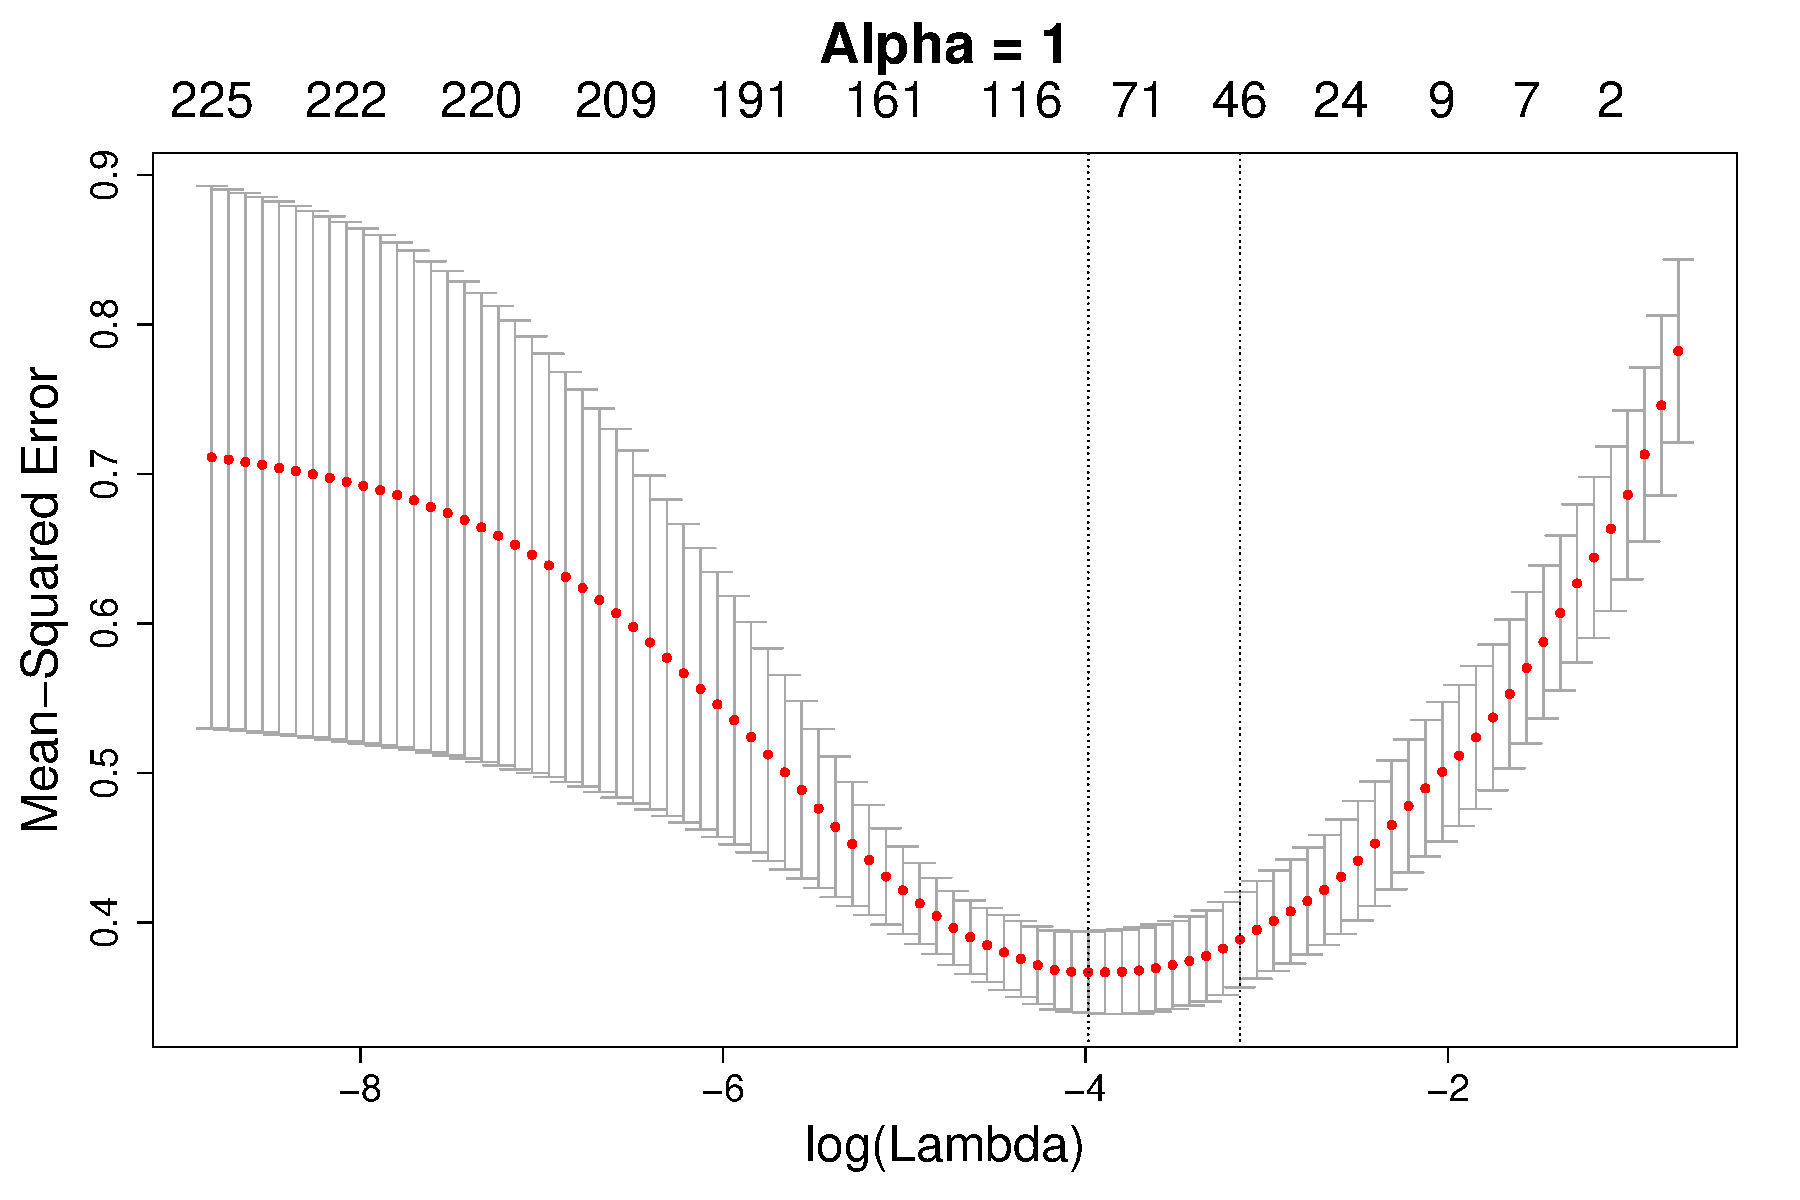
\includegraphics[scale=0.2]{elastic_cv_production}

\end{columns}
\end{frame}

\begin{frame}
\frametitle{Productivity Model - Forward Stepwise}
\begin{columns}

\column{0.5\textwidth}
First 5 variables to enter model
\begin{enumerate}
	\item San Cristobal Island (+)
	\item Percent invasive species (-)
	\item 2 year growth in permanent crops (+)
	\item Percent brush (-)
	\item Growing papaya (+)
\end{enumerate}

\column{0.5\textwidth}
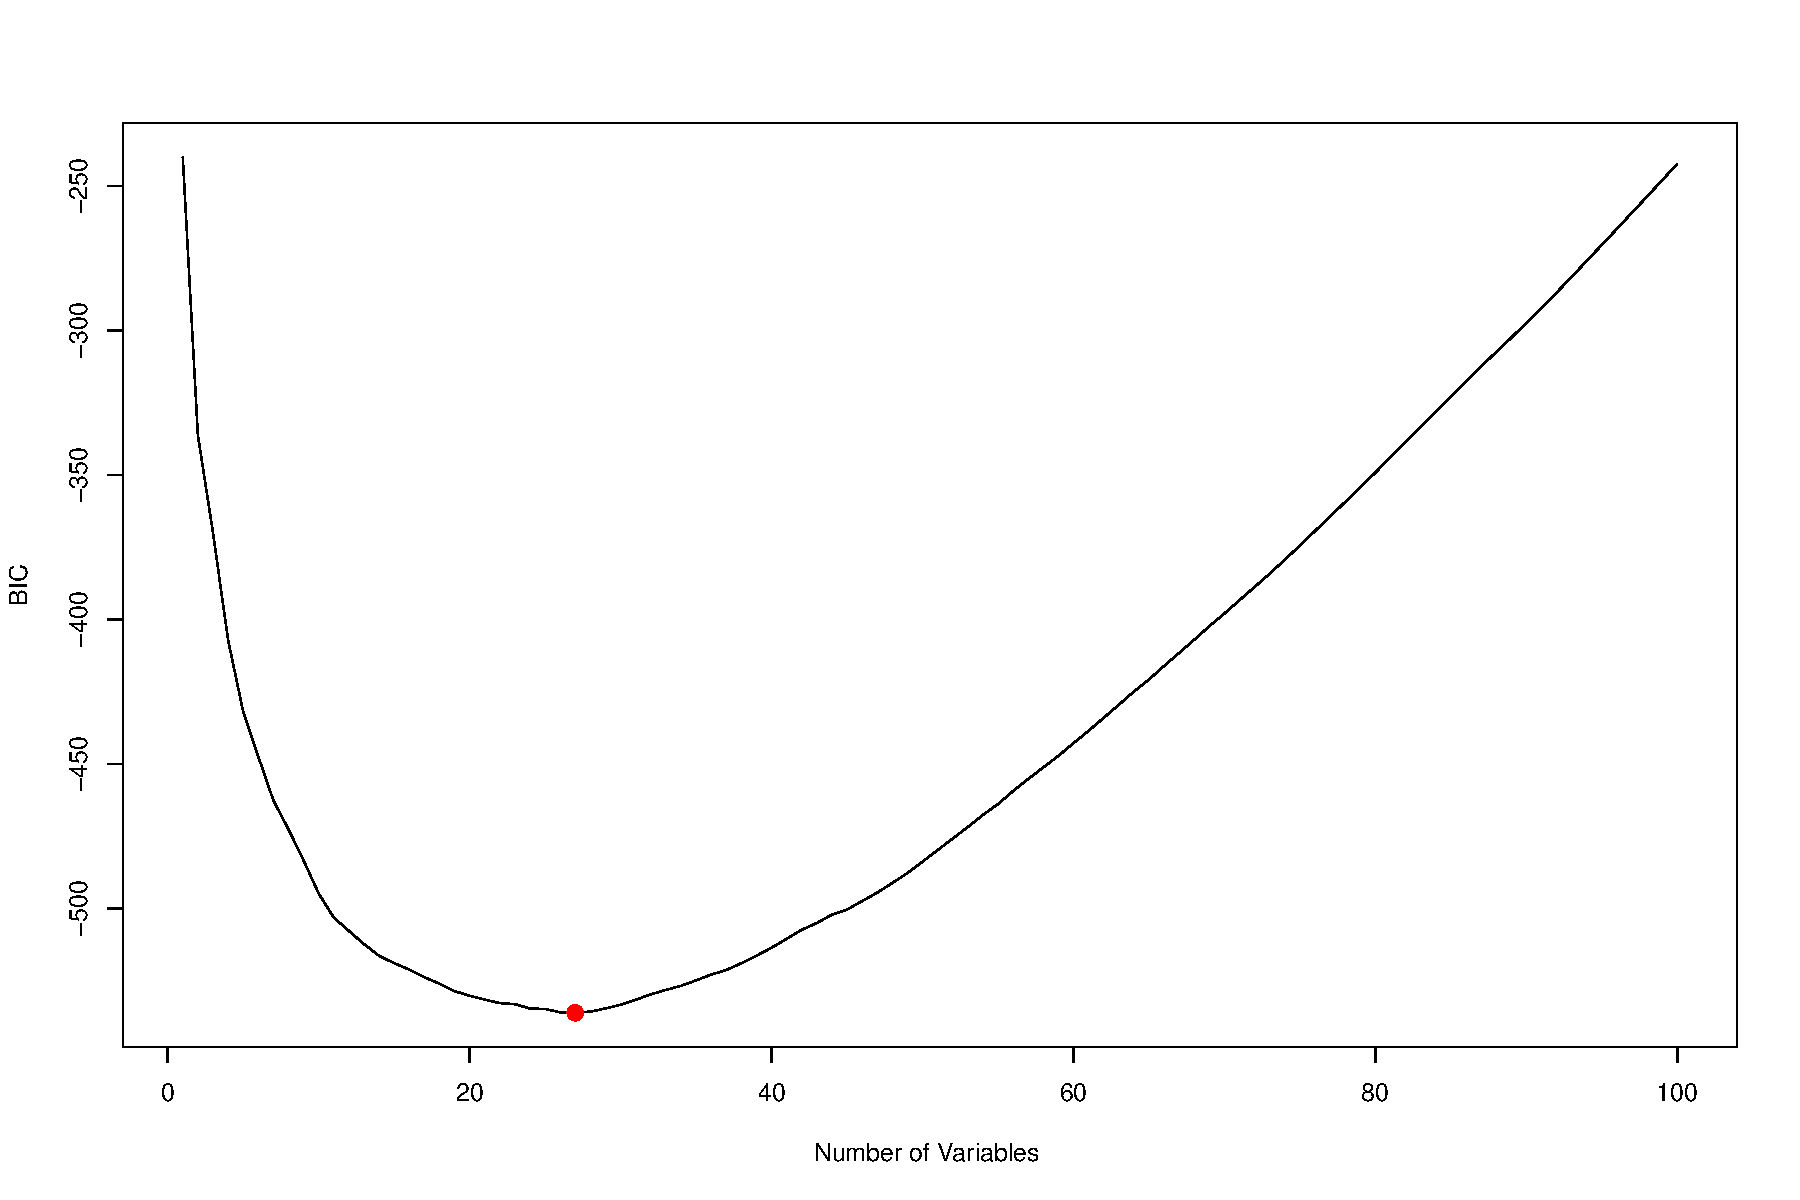
\includegraphics[scale=0.2]{forward_nvars_production}

\end{columns}


\end{frame}

\begin{frame}
\frametitle{Productivity Model - Comparison}
\centering
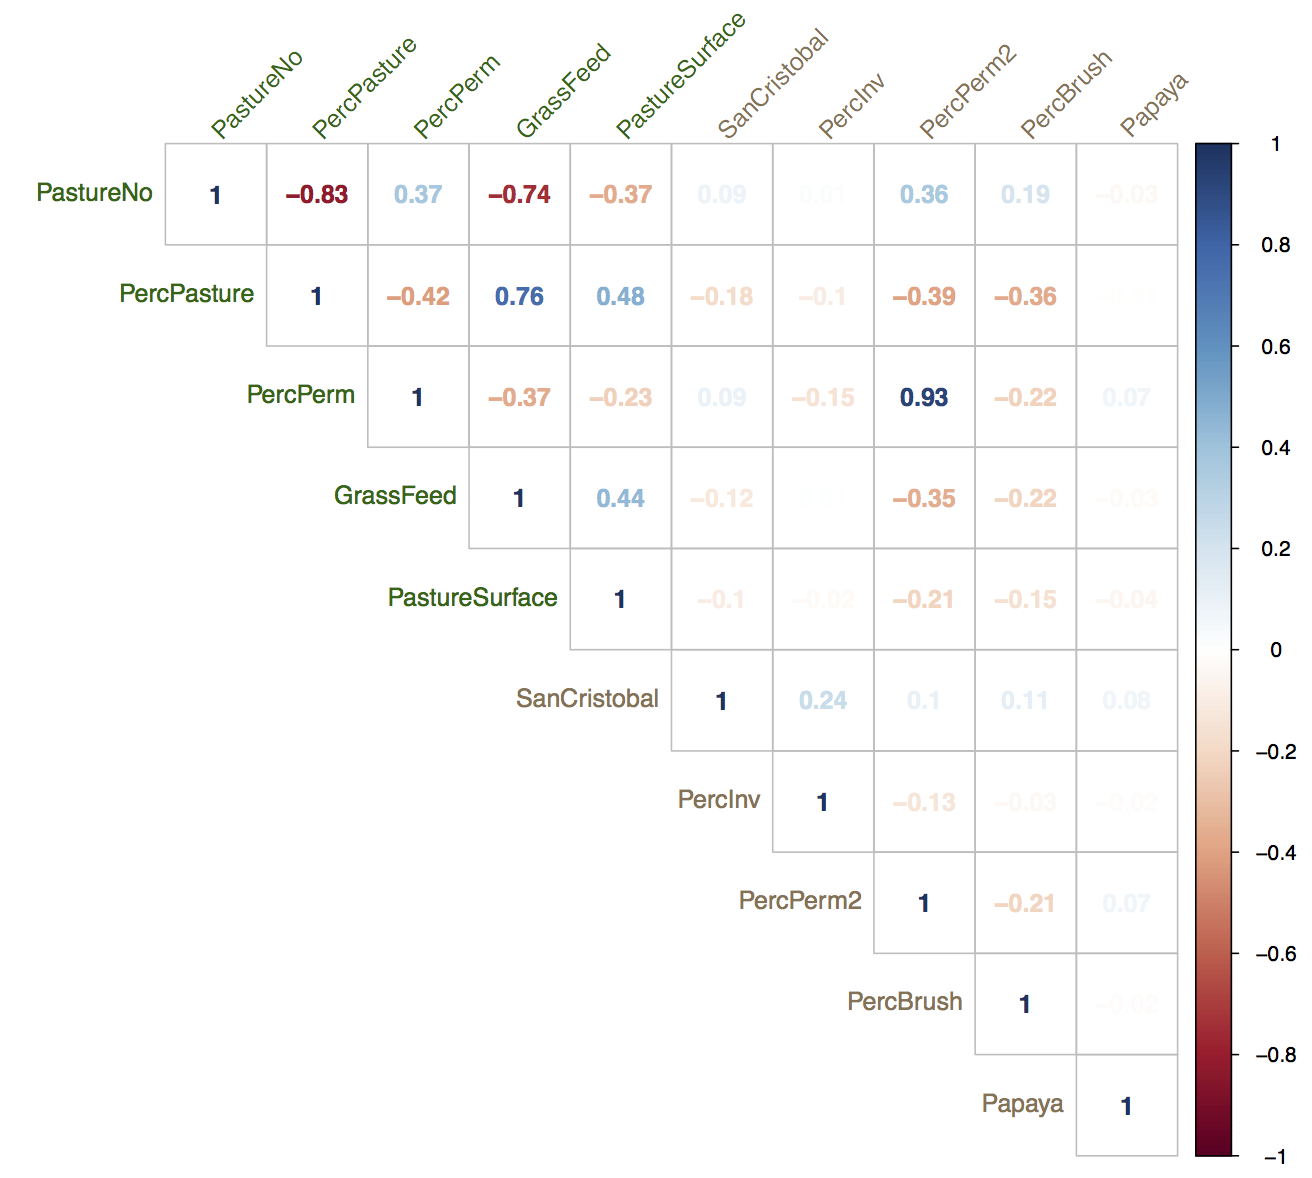
\includegraphics[scale=0.4]{corplot}
\end{frame}

\begin{frame}
\frametitle{Productivity Model - Comparison}
\centering
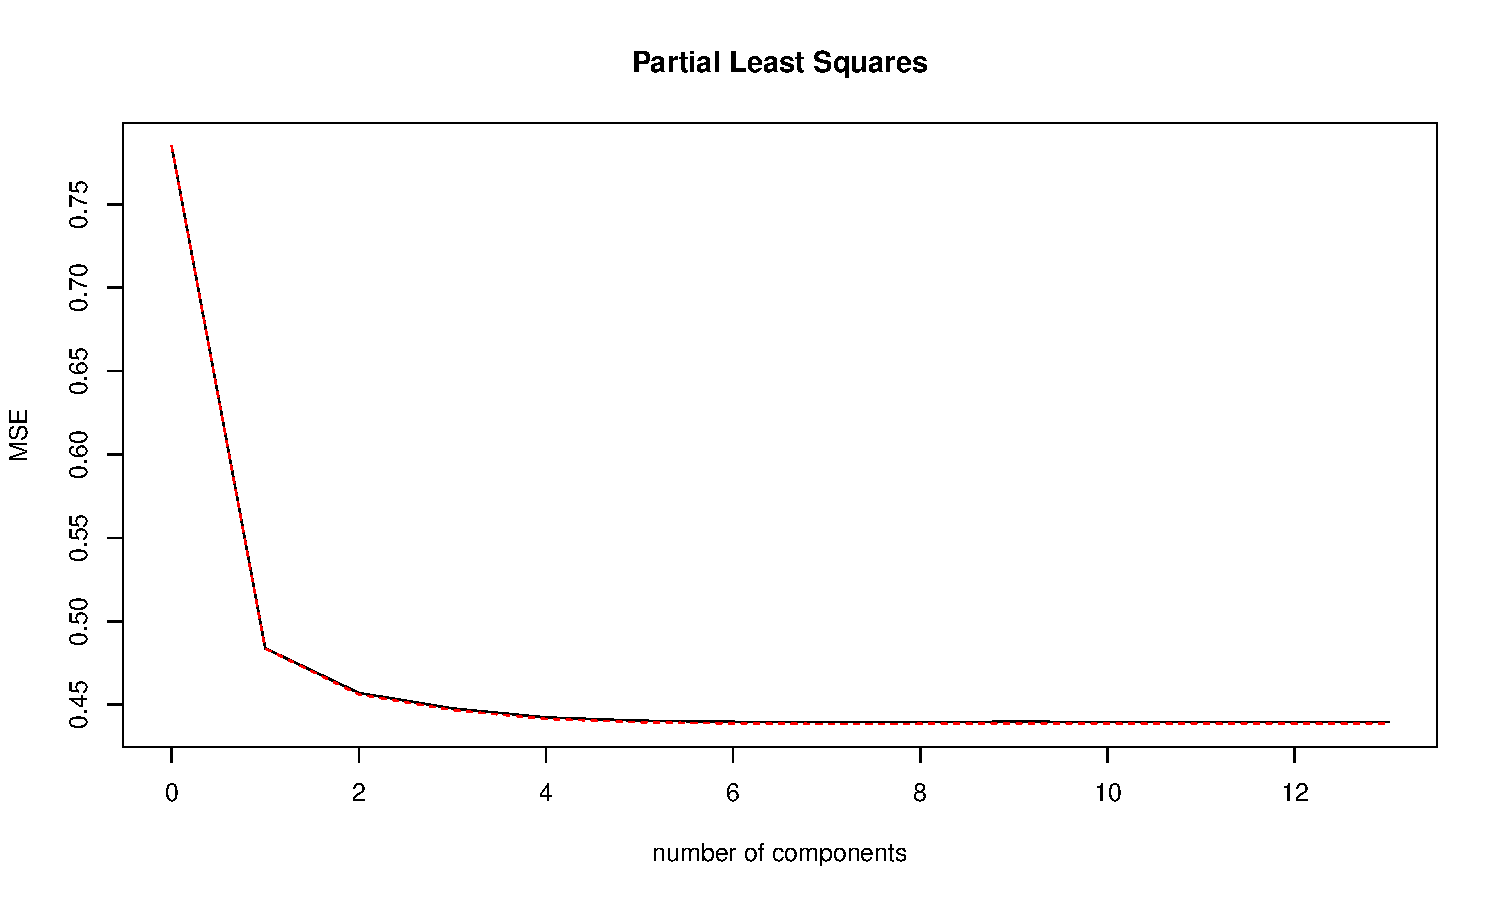
\includegraphics[scale=0.25]{plsplot1}

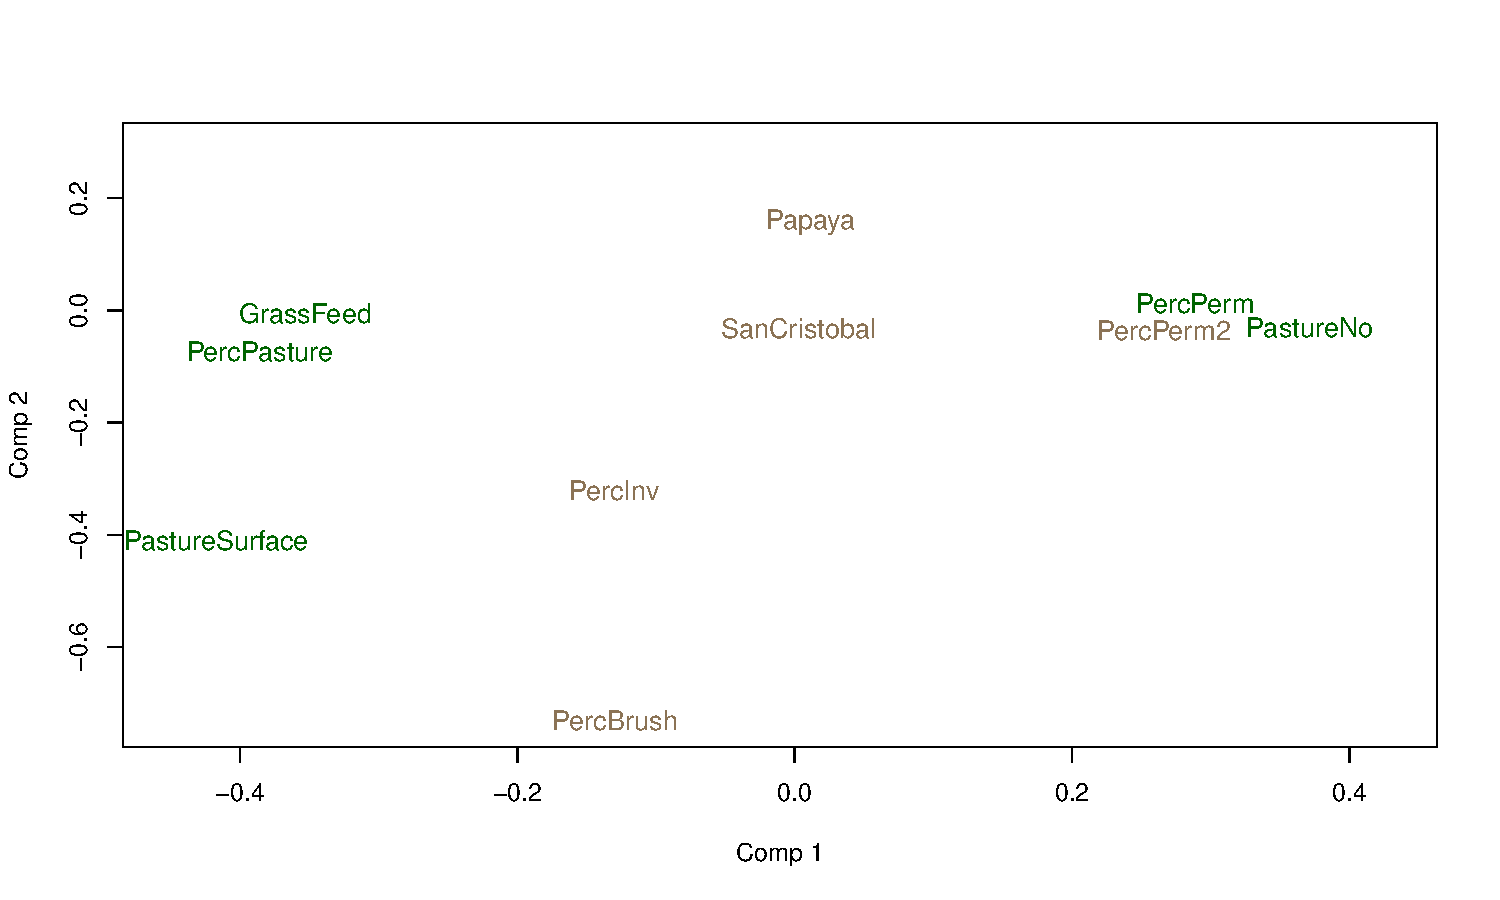
\includegraphics[scale=0.25]{plsplot2}

\end{frame}

\begin{frame}
\centering
{\huge \textbf{Questions?}}

\end{frame}

\end{document}